\section{The Variational Distribution}
\label{sec:var_inference}

The central quantity in Bayesian statistics is the posterior distribution $p(z\mid x)$.
However, in many
nontrivial probabilistic models, including our own, the posterior distribution is intractable to calculate---it requires us to compute the marginal likelihood, $p(x)$, which involves integrating over the latent variable $z$.
In our model, the latent variable space is high dimensional: it is the set of all catalogs. Approximate methods such as MCMC and variational inference are therefore required.

Variational inference~\citep{Jordan_intro_vi, Wainwrite_graph_models_vi, Blei_2017_vi_review} posits a family of distributions $\mathcal{Q}$ and seeks
the distribution $q^*\in \mathcal{Q}$ that is ``closest" to the exact posterior in $\KL$ divergence.
The defined divergence and the family $\mathcal{Q}$ are chosen such that minimizer $q^*$ will
not be too difficult to find via optimization.
We index the distributions in $\mathcal{Q}$ using a real-valued vector $\eta$, in which
case solving for the optimal variational distribution $q_{\eta^*}$
becomes a numerical optimization problem.

% Most commonly, variational inference minimizes the
% \begin{align*}
% \eta^* &= \argmin_{\eta} \mathcal{L}(\eta),
% \end{align*}
% and use $q_{\eta^*}(z \mid x)$ as an approximation to the exact posterior.
%
% Traditionally, variational inference minimizes the negative
% evidence lower bound (ELBO)~\citep{Blei_2017_vi_review},
% \begin{align}
%     \mathcal{L}_{elbo}(\eta) =
%     \Expect_{q_\eta(z \mid x)}\Big[\log p(x, z) - \log q_\eta(z \mid x)\Big].
%     \label{eq:elbo}.
% \end{align}
% Minimizing the negative ELBO is equivalent to minimizing the Kullback-Leibler (KL)
% divergence between $q_\eta(z \mid x)$ and $p(x \mid z)$.
% Computing the ELBO does not require computing the marginal distribution $p(x)$,
% which is intractable, or the posterior distribution $p(z \mid x)$, which would be circular.
Most commonly, variational inference minimizes the ``reverse" KL divergence
between $q$ and $p$:
\begin{align}
   \eta^* &= \argmin_{\eta} \mathrm{KL}\Big[\,q_\eta(z \mid x)\, \| \,p(z \mid x)\,\Big].
   \label{eq:kl_objective}
\end{align}
Minimizing the $\KL$ divergence in~\eqref{eq:kl_objective} is equivalent to maximizing the evidence lower bound (ELBO):
\begin{align}
    \mathcal{L}_{elbo}(\eta) =
    \Expect_{q_\eta(z \mid x)}\Big[\log p(x, z) - \log q_\eta(z \mid x)\Big].
    \label{eq:elbo}
\end{align}
This equality is shown in \cite{Blei_2017_vi_review}. Computing the ELBO does not require computing the marginal distribution $p(x)$, which is intractable, or the posterior distribution $p(z \mid x)$, which would be circular.
In Section~\ref{sec:wake_sleep}, we
consider an alternative objective to \eqref{eq:kl_objective},
where we instead minimize an \textit{expectation}
of the KL divergence with its arguments $q$ and $p$ reversed.


\subsection{Amortized Variational Inference}
We describe the construction of the family $\mathcal{Q}$. 
Traditionally in variational inference, the posterior approximation $q_\eta$ depends on the data $x$ only implicitly,
in that $\eta^*$ is chosen according to~\eqref{eq:kl_objective}.
In this case, $q_\eta(z \mid x)$ is usually written $q_\eta(z)$, suppressing the dependence on $x$.
When a new data point $x^{new}$ arrives, finding a variational  approximation to the posterior $p(z^{new} \mid x^{new})$ requires solving~\eqref{eq:kl_objective} with $x = x^{new}$ through an iterative optimization procedure, which may be computationally expensive.


% The generative model in Section~\ref{sec:gen_model} does not assume any hierarchical structure over replicated  images. Therefore, given a new image $x^{new}$, the posterior factorizes; in other words,
% $p(z^{new}, z \mid x^{new}, x) = p(z^{new} \mid x^{new}) p(z \mid x)$.
% To find a variational  approximation to the posterior $p(z^{new} \mid x^{new})$, the optimization problem~\eqref{eq:kl_objective} must be solved again with $x = x^{new}$.
% Even in models with hierarchical structure, the variational distribution will generally need to be updated via optimization for every newly observed data point.

On the other hand,
in {\itshape amortized} variational
inference~\citep{kingma2013autoencoding, rezende2014stochastic}, $q_\eta$ is an explicit function of the data.
In our case, this means a flexible, parameterized function maps input $x$, an observed image, to a real-valued vector characterizing a distribution on the latent space $\mathcal{Z}$.
Typically, the function is a neural network, in which case the variational parameters $\eta$ are the neural network weights.
After the neural network is fitted using a collection of observed $x$'s, the approximate posterior $q_\eta(z^{new} \mid x^{new})$ for a new data point
$x^{new}$ can be evaluated with a single forward pass through the neural network.
No additional run of an optimization routine is needed for a new data point $x^{new}$.

The following subsections detail the construction of our variational distribution, which will 
be fitted in an amortized fashion. 


\subsection{The Factorization}
\label{sec:factorization}

% \begin{wrapfigure}{r}{0.35\textwidth}
%     \centering
%     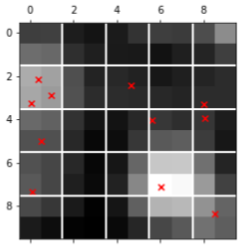
\includegraphics[width = 0.32\textwidth]{figures/vi_figures/example_tiled_less_whitespace.png}
%     \caption{Tiling a $10 \times 10$ pixel image into $2 \times 2$ tiles.}
%     \label{fig:ex_tiles}
% \end{wrapfigure}

\begin{figure}[tb]
    \centering
    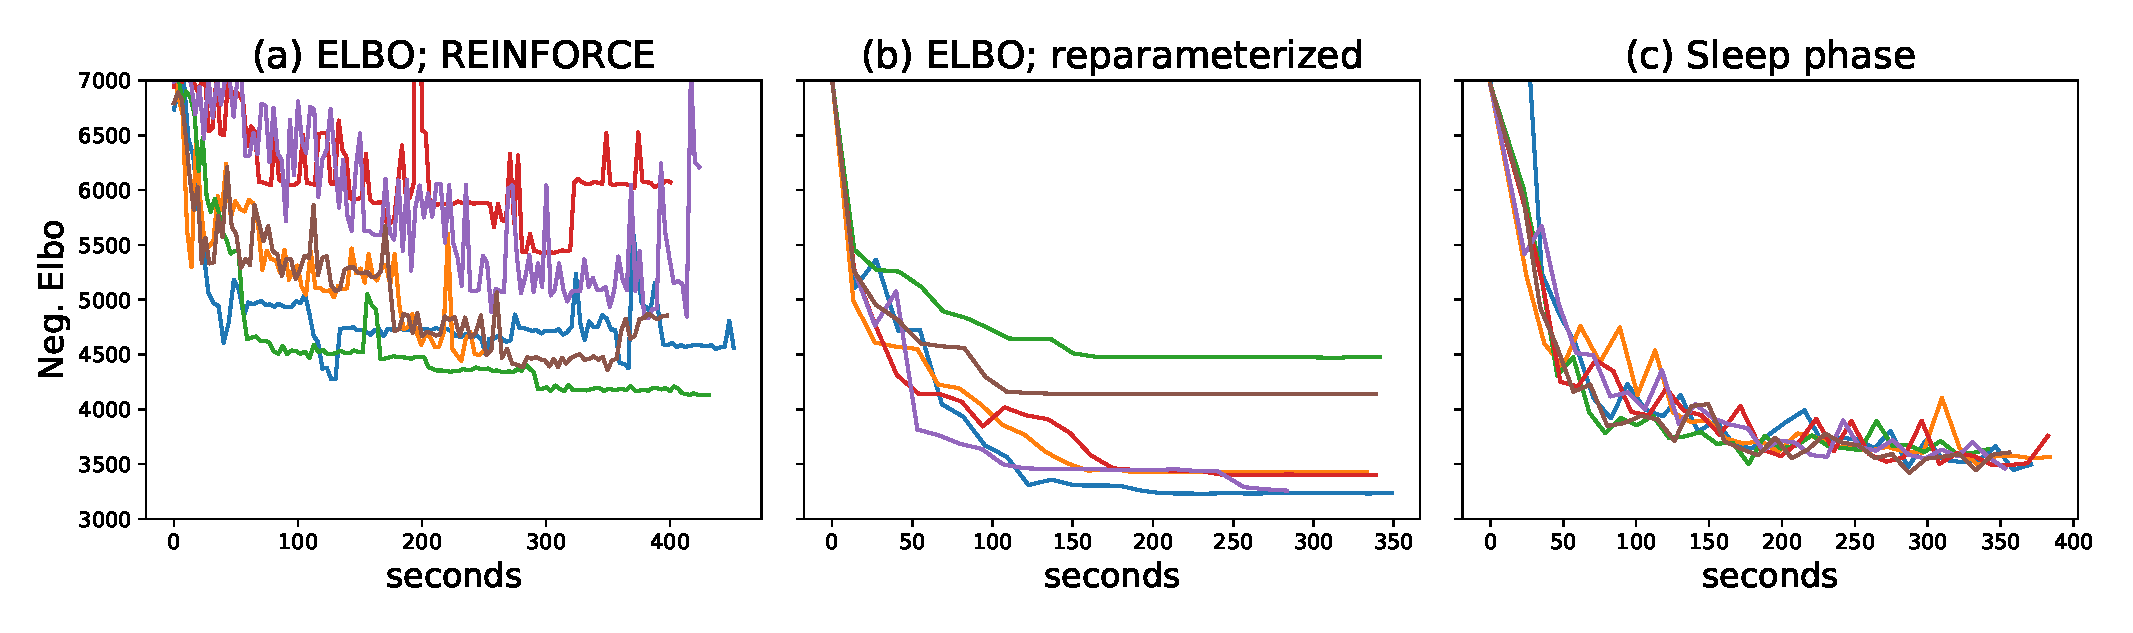
\includegraphics[width = 0.25\textwidth]{figures_vg/vi_figures/example_tiled_10.eps}
    \caption{Tiling a $20 \times 20$ pixel image into four $10 \times 10$ tiles.}
    \label{fig:ex_tiles}
\end{figure}

To make optimization tractable, the family $\mathcal{Q}$ is normally restricted to probability distributions
without conditional dependencies between some latent variables. In the most extreme case, known as mean-field variational inference, the variational distribution completely factorizes across all latent variables.

Our factorization has a spatial structure.
First, we partition the full $H \times W$-pixel image into disjoint $R \times R$-pixel tiles.
$R$ is chosen such that the probability of having three or more stars in one tile is small.
In this way, the cataloging problem decomposes to inferring only a few stars at a time (Section~\ref{sec:nn_architecture}).


Let $S = \sfrac{H}{R}$ and $T = \sfrac{W}{R}$ and assume without loss of generality that $H$ and $W$ are multiples of $R$.
For $s = 1, ..., S$ and $t = 1, ..., T$,
the tile $\tilde x_{st}$ is composed of the pixels
\begin{align}
    \tilde x_{st} = \{x_{hw} : Rs \leq h < R(s+1) \text{ and } Rt \leq w < R(t+1)\}.
    \label{eq:tiles}
\end{align}
Figure~\ref{fig:ex_tiles} gives an example with $R = 2$.

Let $\tilde N^{(s, t)}$ be the number of stars in tile $(s,t)$.
Because $\tilde N^{(s, t)}$ is random,
the cardinality of the set of locations and fluxes in each tile
is also random.
To handle the trans-dimensional parameter space,
we consider {\itshape triangular arrays} of latent variables
for each tile:
\begin{align}
    \tilde\ell^{(s, t)} &= (\tilde\ell_{N, i}^{(s, t)} : i = 1, ..., N; N = 1, 2, ...), \\
    \text{ and } \tilde f^{(s, t)} &= (\tilde f_{N, i}^{(s, t)} : i = 1, ..., N; N = 1, 2, ...),
\end{align}
where $\tilde\ell_{N, i}^{(s, t)}$ and $\tilde f_{N, i}^{(s, t)}$ are the elements of the triangular array corresponding to location and fluxes, respectively.
Tile locations $\tilde\ell_{N, i}^{(s, t)} \in [0, R]\times[0, R]$ give the location of stars within a tile. The fluxes $\tilde f_{N, i}^{(s, t)}$ are vectors in $\mathbb{R}^B_+$ (one flux for each band).

We refer to $(\tilde N^{(s, t)}, \tilde \ell^{(s, t)}, \tilde f^{(s, t)})_{s=1,t=1}^{S,T}$ as the {\itshape tile latent variables}. The distribution on tile latent variables factorize over image tiles:
\begin{align}
    \tilde q_\eta\big( \big(\tilde N^{(s, t)}, \tilde \ell^{(s, t)}, \tilde f^{(s, t)}\big)_{s=1, t = 1}^{S, T} \mid x\big)
    &=
    \prod_{s = 1}^S \prod_{t=1}^T
    \tilde q_\eta\big(\tilde N^{(s, t)}, \tilde \ell^{(s, t)}, \tilde f^{(s, t)} \mid x\big).
    \label{eq:factorize_patches}
\end{align}

We denote tile latent variables as $\tilde z$.
The ultimate latent variable of interest is $z = \{N, (\ell_i, f_{i,1}, ..., f_{i,B})_{i = 1}^N\}$, the catalog for the full image.
There is a mapping from $\tilde z$ to $z$.
First, the number of stars in the full catalog is given by the sum of the stars in each tile, $N = \sum_{s,t} \tilde N^{(s, t)}$.
Then, for every tile $(s,t)$, we index into the $\tilde N^{(s,t)}$-th row of the triangular array of tile latent variables $\tilde f^{(s,t)}$ and $\tilde \ell^{(s,t)}$.
The union of these fluxes and locations over all tiles form the full catalog (tile locations are shifted by the position of the tile in the full image to obtain locations in the full image).
See Figure~\ref{fig:tile_to_full_schm} for a schematic.


% \begin{align}
%     \{f_i\}_{i=1}^N = \Big\{\tilde f_{\tilde N^{(s, t)}, i}^{(s, t)} : i = 1, ..., \tilde N^{(s, t)}, s = 1, ..., S, t = 1, ..., T \Big\},
% \end{align}
% and the corresponding locations are
% \begin{align}
%     \{\ell_i\}_{i = 1}^N = \left\{\tilde \ell_{N^{(s, t)}, i}^{(s, t)} +
%     \begin{pmatrix}
%     Rs \\ Rt
%     \end{pmatrix}
%     : i = 1, ..., N^{(s, t)}, s = 1, ..., S, t = 1, ..., T\right\}.
% \end{align}
% The tile location is shifted by $(Rs, Rt)$ to obtain the location in the full image.

% Given this mapping from tile latent variables to the catalog of interest,
% \begin{align}
%  \big(\tilde N^{(s, t)}, \tilde \ell^{(s, t)}, \tilde f^{(s, t)}\big)_{s=1, t = 1}^{S, T}
% \mapsto
% \{N, (\ell_i, f_{i,1}, ..., f_{i,B})_{i = 1}^N\},
% \label{eq:patch_to_full_map}
% \end{align}
% a distribution on the tile latent variables induces a distribution on catalogs.

% Within each tile $(s,t)$, the distribution also fully factorizes:
% \begin{align}
%     \tilde q_\eta\big(\tilde N^{(s, t)}, \tilde \ell^{(s, t)}, \tilde f^{(s, t)} \mid x\big)
%     &=
%     \tilde q_\eta\big(\tilde N^{(s, t)} \mid x\big)
%     \prod_{n = 1}^\infty \prod_{i = 1}^n
%     \tilde q_\eta\big(\tilde \ell_{n,i}^{(s, t)} \mid x\big)
%     \tilde q_\eta\big(\tilde f_{n,i}^{(s, t)} \mid x\big).
%     \label{eq:factorize_within_patch}
% \end{align}

If $\tau$ is the mapping from $\tilde z$ to $z$,
then the variational distribution on catalogs $z$ is
\begin{align}
    q_\eta(z \mid x) := \tilde q_\eta(\tau^{-1}(z) \mid x),
    \label{eq:pull_back_of_q}
\end{align}
where $\tau^{-1}(z)$ is the pre-image of $z$ under $\tau$.
See Appendix~\ref{sec:eval_var_distr} for details on evaluating $q_\eta(z \mid x)$ for any given catalog $z$, which by \eqref{eq:pull_back_of_q} requires finding the pre-image $\tau^{-1}(z)$.


% for the figure
% {\color{blue} \tilde N^{(1,1)} = 2}

% \\

% \\

% \begin{pmatrix}
% (\tilde \ell, \tilde f)_{1, 1} & \\
% \color{blue} (\tilde \ell, \tilde f)_{2, 1} &
% \color{blue} (\tilde \ell, \tilde f)_{2, 2} &
% \end{pmatrix}^{(1,1)}

% \{{\color{Blue} N = 4},
% {\color{red} (\tilde \ell, \tilde f)^{(1,1)}_{2,1},
% (\tilde \ell, \tilde f)^{(1,1)}_{2,2}},
% {\color{DarkGreen} (\tilde \ell, \tilde f)^{(1,2)}_{1, 1}},
% {\color{Orange} (\tilde \ell, \tilde f)^{(2,1)}_{1, 1}}
% \}

\begin{figure}[tb]
    \centering
    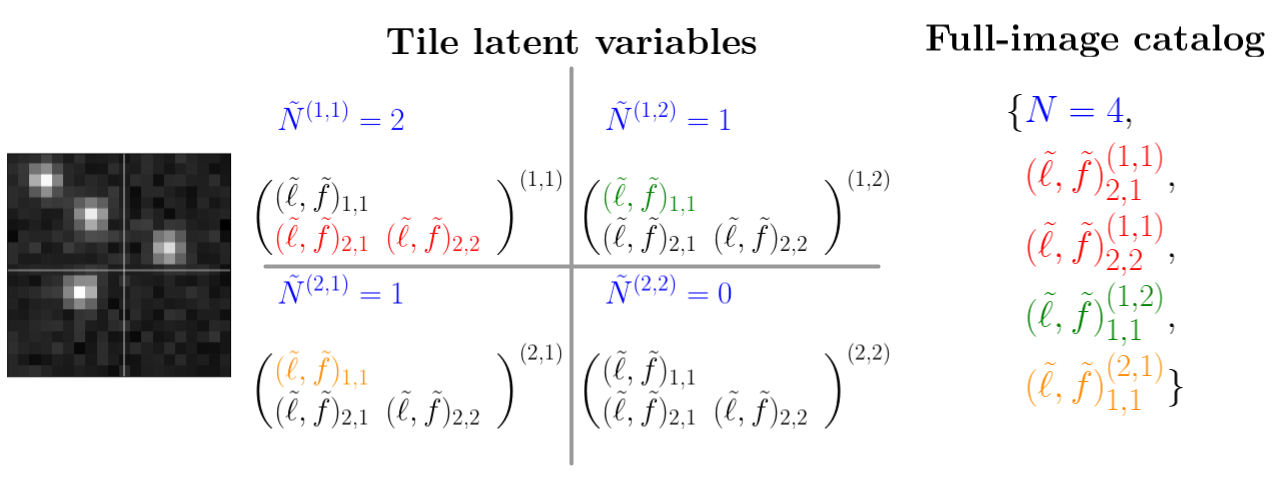
\includegraphics[width = 0.9\textwidth]{figures/vi_figures/tile_to_full_schematic.png}
    %\vspace{-0.6cm}
    \caption{An example image with four tiles and four stars illustrating the relationship between the tile latent variables and the full-image catalog.
    To construct the full-image catalog, we index into the appropriate row of the triangular array for each tile.}
    \label{fig:tile_to_full_schm}
\end{figure}


\subsection{Variational Distributions on Image Tiles}
\label{sec:distr_on_tiles}
We describe the variational distribution for each tile,
$\tilde q_\eta\big(\tilde N^{(s, t)}, \tilde \ell^{(s, t)}, \tilde f^{(s, t)} \mid x\big)$.
The latent variables fully factorize within each tile.
Dropping the index
$(s,t)$ in this subsection,
\begin{align}
    \tilde N &\sim \text{Categorical}(
    \omega; 0, ..., N_{max});  \label{eq:var_distr_n}\\
	\tilde \ell_{j, i} / R &\sim \text{LogitNormal}(\mu_{\ell_{j, i}}, \text{diag}(\nu_{\ell_{j, i}}) )\label{eq:var_distr_loc}; \\
	\tilde f^b_{j, i} &\sim \text{LogNormal}(\mu_{f^b_{j, i}}, \sigma^2_{f^b_{j, i}}), \label{eq:var_distr_f}
\end{align}
independently for $i = 1, ..., j$; $j = 1, ..., N_{max}$.
Here $\omega$ is a $(\tilde N_{max} + 1)$-dimensional vector on the simplex. $\mu_{\ell_{j, i}}$ and $\nu_{\ell_{j, }}$ are two-dimensional vectors---the covariance on locations is diagonal.
Note that in the exact posterior, $\tilde N$ has support on the nonnegative integers, whereas in the variational distribution $\tilde N$ is truncated at some large $N_{max}$.


These distributions were taken to match the constraints of the latent variables: fluxes are positive and right skewed, suggesting a log-normal; locations are between zero and $R$, suggesting a scaled logit-normal.

\subsection{Neural Network Architecture}
\label{sec:nn_architecture}

In each tile, the distributional parameters in \eqref{eq:var_distr_n},
\eqref{eq:var_distr_loc}, and \eqref{eq:var_distr_f} are the output of a neural network.
The input to the neural network is an $R \times R$ tile, padded with surrounding pixels.
Padding enables the neural network to produce better predictions inside the tile.
For example, a bright source outside but in the vicinity of the tile affects the pixel values inside the tile.
Padding the tiles allows the neural network access to this information.
Thus, while the distribution on tile latent variables factorize over tiles, the neural network is able to use information from neighboring tiles in producing the distributional parameters.

The appropriate amount of padding will depend on the PSF width in the analyzed image.
To catalog the crowded starfield M2 (Section~\ref{sec:results_on_m2}),
we set $R = 2$ and padded the tile with a three-pixel-wide boundary.
In cataloging a DECam image, we use larger tiles with more padding because the width of the PSF is larger in these images. There, we set $R = 10$ and used a five-pixel-wide boundary.


% Let $\hat x^{(s,t)}$ denote the padded tile pixel intensities (which includes all $B$ bands) and $h_\eta$ be the neural network.
% which returns the collection of distributional parameters %in~\eqref{eq:var_distr_n}-\eqref{eq:var_distr_f} on tile $(s,t)$.
% \begin{align}
%     h_\eta(\hat x^{(s,t)}) = (\omega^{(s,t)}, \mu_\ell^{(s,t)}, \nu_{\ell}^{(s,t)}, \mu_f^{(s,t)}, \sigma^{(s,t)}_f).
%     \label{eq:nn_output}
% \end{align}
% The same neural network is evaluated for all tiles $(s,t)$.
In amortized inference, the variational parameters $\eta$ are neural network weights.
The architecture consists of a convolutional layer followed by several residual network layers, which themselves contain convolutions, before ending with several fully connected layers (Figure~\ref{fig:starnet_arch}).
This architecture has been successful on image classification challenges such as ImageNet~\citep{imagenet2015}.
We tuned the architecture using Optuna, an automatic hyper-parameter optimization package \citep{optuna_2019}. 
Our search included the number of convolution layers, 
the number of fully connected layers,
the number of channels in the convolution layers, and the size of the fully connected layers. 

An input to the network is a padded tile, which consists of $B$ color bands. 
We also append an additional ``band" to the input, which 
is a one-hot encoding with
ones for pixels inside the tile, and zeros outside. 
We do this because the network is only responsible for inferring sources inside each tile, and this additional band gives
the network access to a feature which encodes the tile interior. 

See Appendix~\ref{sec:supp_nn_architecture} for further details 
concerning the parameters of our neural network architecture. 
% our focus in this paper is the application of neural networks to provide a variational posterior for cataloging starfields, not the network architecture per se.


% Convolutional layers are useful for localizing stars, as they make the network invariant to shifts in stellar location. The convolutional kernel in the first layer is $3\times3$ pixels, roughly the full width at half maximum (FWHM) of the PSF.

\begin{figure}[!tb]
    \centering
    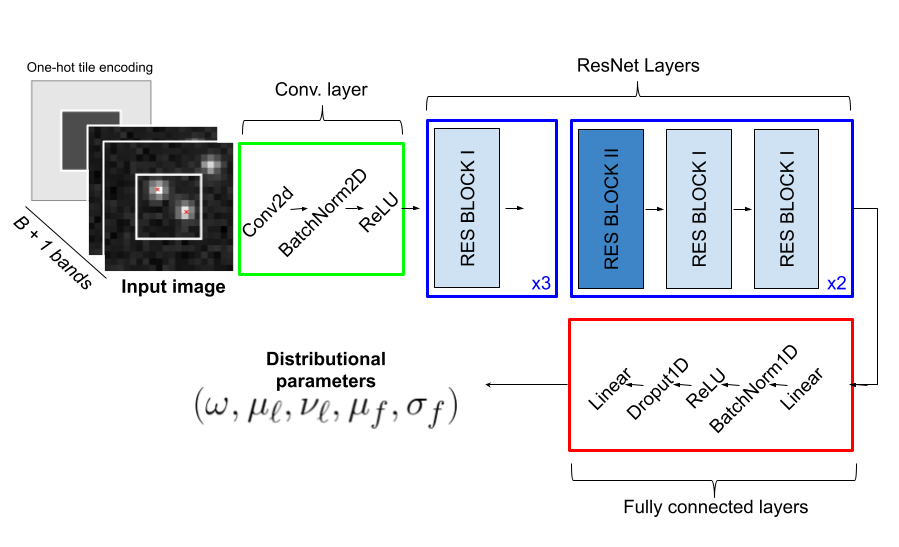
\includegraphics[width=\textwidth]{figures_vg/starnet_archetecture9.png}
%    \vspace{-1.cm}
    \caption{The neural network architecture. The DECam input is a two-band $20\times 20$ padded tile, 
    and the network returns distributional parameters corresponding to sources located in the $10\times 10$ tile outlined in white.
    In this example, there are two sources located in the $10\times10$ tile.
    The additional input band is a one-hot encoding with ones for pixels inside the tile, and zeros outside. 
    For further details concerning the residual network blocks (in blue), see 
    Appendix~\ref{sec:supp_nn_architecture}.
    }
    \label{fig:starnet_arch}
\end{figure}

% Note the output dimension of the neural network. For each tile $(s,t)$, the categorical parameter $\omega^{(s,t)}$
% lies on the simplex and has dimension $N_{max} + 1$.
% Furthermore, each index of the triangular array
% $i = 1, ..., \tilde N^{(s,t)}$, $\tilde N^{(s,t)} = 1, ..., N_{max}$
% describes a star. The star has a mean and variance for each location coordinate, and a mean and variance for its flux in each band.
% Thus, for each star $(\tilde N^{(s,t)}, i)$,
% the neural network outputs $2 \times (B + 2)$ parameters.
% In total, the neural network has output dimension $(N_{max} + 1) + (B + 2) \times (N_{max}^2 + N_{max})$.

% Recall that locations on the
% full image $\ell_{N, i}$ are parameterized to be in $[0, H] \times [0, W]$.
% On the tiles, locations $\ell^{(k)}_{N, i}$ are parameterized to be in
% $[0, s] \times [0, s]$.

Note that the output dimension of the neural network is quadratic in $N_{max}$: the outputs are parameters for a triangular array consisting of $\frac{1}{2}(N_{max}^2 + N_{max})$ sources.
Factorizing the variational distribution spatially keeps the output dimension manageable.
While the full image may contain many stars
(on the images that we catalog, the number of stars is on the order of thousands),
we set $N_{max} = 3$ for each tile.
Thus, the network is responsible for inferring only a few stars at once---a much easier task than inferring all stars simultaneously.

We emphasize that while the variational distribution factorizes over tiles, our method does not break the inference problem for the full image into isolated subproblems.
The likelihood of the full image does not factorize over tiles. Light from a star within a tile spills over into neighboring tiles, so the likelihood should not and does not decouple across image tiles.
